\setchapterpreamble[u]{\margintoc}
\chapter{Enriching the classic TTO formulation with advanced mechanical constraints}
Introduction
\todo{check the word paper}
\todo{every eq and fig must begin with the chapter}
\todo{scaling images}

\begin{table*}[]
    \centering
    \begin{tabular}{V{4cm}
        V{2.5cm}
        V{2.5cm}
        V{2.5cm}
        V{2.5cm}
        V{2.5cm}}
        \toprule
    Authors &
      Stress &
      Local Buckling &
      Topological buckling &
      Kinematic compatibility &
      Multi-load cases
       \\ \midrule
    Dorn et al. (1964)                  & x &-&-&-&-\\
    Hemp (1973)                         & x &-&-&-& x \\
    Reinschmidt et al.   (1974)         & x & x &-& $\sim$ &-\\
    Kirsch (1980)                       & x &-&-& x &-\\
    Oberndorfer et al. (1996)           & x & x &-&-&-\\
    Silva Smith (1997)                  & x & x & $\sim$ &-& x \\
    Achtziger (1999a, 1999b)            & x & x & x &-& x \\
    Stolpe (2004)                       & x & x &-& x & x \\
    Pritchard et al. (2005)             & x &-&-&-& x \\
    Tyas et al. (2006)                  & x & x & x &-& x \\
    Descamps et al. (2014)              & x & x & x &-& x \\
    Schwarz et al. (2018)               & x & x &-&-&-\\
    Cai et al. (2022)                   & x & x & x &-&-\\
    Present work                        & x & x & x &x&x\\ \bottomrule
    \end{tabular}
    \caption{Non-exhaustive list of the existing research in Truss Topology Optimization (TTO) with their corresponding scientific contributions}
    \label{tab:}
    \end{table*}

\section{Advanced mechanical constraints}


\subsection{Minimum slenderness constraints}
As previously discussed in \secref{sec:03_applications}, the \gls{tto} method has limitations due to its reliance on the truss model. Consequently, we cannot rely on the results if the model falls outside the bounds of this idealization. To better study this limit, as outlined in \secref{sec:03_applications}, we introduced a metric called bar slenderness defined as follows:
\begin{equation}
    \lambda = \frac{\ell}{R_{\mathrm{g}}},
\end{equation}
where $R_{\mathrm{g}}$ represent the gyration radius of the cross-sectional area, defined as $R_{\mathrm{g}} = \sqrt{I/a_j}$.
The primary objective of this section is to introduce an upper limit constraint on the cross-sectional area design variable. This constraint prevents a bar from exceeding the bounds of its idealized model, thereby enhancing the optimization process's robustness.

Remembering that for a circular cross-section $I = \pi r_j^4/4$, we can write
\begin{equation}
    R_{\mathrm{g},j} = \frac{r_j}{2}.
\end{equation}
The minimum slenderness limit constraints are then stated as:
\begin{equation} \label{eq:04_slend_constraints}
    a_j \leq \frac{4 \pi \ell_j^2}{\lambda_{\text{max}}}, \quad \forall j \in [1,\ldots, N_{\text{el}}]
    \tag{$\vect{g}_{\text{slend}}$}
\end{equation}
for a fixed $\lambda_{\text{max}}$. In this thesis we set $\lambda_{\text{max}}=15$.

\subsection{Local and topological buckling constraints}
Adding local buckling constraints to the optimization formulation is fundamental, as ultralight truss structures are often dominated by this mode of failure \sidecite{sigmund_non-optimality_2016}. By imposing local buckling constraints over a \gls{tto} problem (where the lower bound for the members' cross-sectional areas is 0), the optimization domain becomes disjointed \sidecite{cheng_aspects_1995}. The solution is to be searched inside a degenerate space of the design space of the optimization, known in the literature as singular optimum \sidecite{guo_new_2001}. Stolpe \sidecite{stolpe_note_2003} showed how using the \gls{sand} formulation with local buckling and kinematic compatibility constraints, it is possible to find well-optimized structures without the use of relaxation techniques. The authors, however, point out how the solution is still very sensitive to the initialization point of the \gls{nlp} formulation. The local buckling constraints $\vect{g}_{\text{buck}}$ are stated using Euler's critical load formula as:
\begin{equation}
    q_j  + \frac{s_j a_j^2}{\ell_j^2} \geq 0 \quad \forall j \in [1,\ldots, N_{\text{el}}],
    \tag{$\vect{g}_{\text{buck}}$}
    \label{eq:buck}
\end{equation}
where $s_j$ is a parameter dependent on the member material and section topology as follows:
\begin{equation}
    s_j=\pi^2 E \beta_j.
    \label{eq:s}
\end{equation}
$\beta_j=I_j/a^2_j$ is a positive constant dependent on the moment of inertia and the section of the $j$-th bar, and $E$ is Young's modulus of the material. Assuming that the shape of the cross-section is identical over the whole structure and is independent of $a$, it follows that  $\beta_j = \beta$ and $s_j = s, \; \forall j \in [1,\ldots, N_{\text{el}}]$.

Direct application of the local buckling constraint \eqrefnotext{eq:buck} in the optimization formulation tends to create "chains" of unstable compressive members \sidecite{bendsoe_optimization_1995, zhou_difficulties_1996, rozvany_difficulties_1996}. This problem is known in the literature as topological buckling \sidecite{achtziger_local_1999}, as the definition of the compressive chains is a function of the topology of the structure, and is one of the elements of the nodal stability of the structure. Additional forms of structure instability, such as global buckling \sidecite{ben-tal_optimal_2000,kocvara_modelling_2002} or the use of lateral perturbing forces to obtain nodal stability \sidecite{tyas_practical_2006,mela_resolving_2014} have been studied in the literature. However, since they are beyond the scope of this work, they will not be discussed further.

\begin{figure}
    \centering
    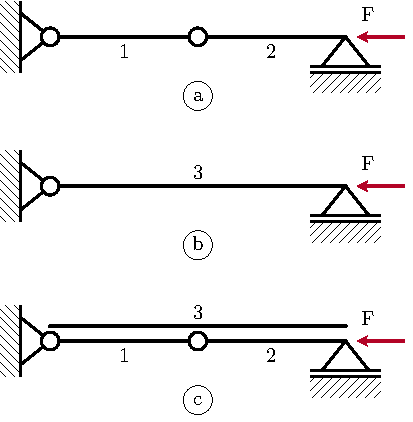
\includegraphics[width=0.5\textwidth]{figures/04_TTO_improvements/01_3_bars_chain/3_bars_chain.pdf}
    \caption{The three ground structures loaded in compression are used to highlight the topological buckling problem in \gls{tto}. (a) Two-bar ground structure loaded in compression; (b) single bar ground structure; (c) overlap of the $a$ and $b$ ground structures.}
    \label{fig:chain_buck}
\end{figure}

To illustrate the topological buckling phenomenon, we consider the case shown in \figref{fig:chain_buck}a. It consists of a ground structure with $M=3$ nodes and $N_{\text{el}}=2$ bars with length $\ell_1=\ell_2=\ell$, and a compressive load of magnitude $F$ applied at the right-hand side node. For this trivial structure, we can state that $q_1=q_2=F$ and thus $a_1=a_2=a$. We suppose here that the allowables of the material are such that the local buckling (and not the stress) is the most limiting failure criterion for the bars. Assuming that the shape of the section is equal, the local buckling constraints are written as:
\begin{equation}
    q_j\geq -\frac{s a^2}{\ell^2}, \quad j\in[1,2].
    \label{eq:chain_1}
\end{equation}
However, the structure is unstable because the vertical force equilibrium equation evaluated on the central hinge is satisfied only in an ideal case where no structural imperfections are taken into account.

If the hinge between bars 1 and 2 is deleted, we obtain the structure pictured in \figref{fig:chain_buck}b with $\ell_3=2\ell$. The local buckling constraints for bar 3 are thus:
\begin{equation}
    q_3\geq -\frac{s a_3^2}{(2\ell)^2}.
    \label{eq:chain_2}
\end{equation}

Combining \eqsref{eq:chain_1}, \eqrefnotext{eq:chain_2} and observing that $q_1=q_2=q_3=F$, it is now trivial to demonstrate that $a_3=2a$. Constraint \eqrefnotext{eq:chain_2} leads, then, to more voluminous structures compared to constraint \eqrefnotext{eq:chain_1}. For that reason, even if we consider the ground structure given in \figref{fig:chain_buck}c composed by the superposition of the ground structures in \figref{fig:chain_buck}a and \figref{fig:chain_buck}b, the optimization with a uniform initialization tends to converge to the solution $\vect{a}^*=[a,a,0]$, unstable but lighter than the physical solution $\vect{a}_p^*=[0,0,2a]$. 

The easiest way to get rid of the instability of the compressive chains is to post-process the optimized structure to remove the unstable hinges between the compressive bars. Doing that, the local buckling constraints are not satisfied anymore as the effective buckling length has increased. It is, then, necessary to calculate the section of the new compressive bars to comply with the newly introduced buckling constraints. As extensively shown by Achtziger \sidecite{achtziger_local_1999b}, this post-processing phase leads to structures that are less optimal compared to the ones we could obtain if we take into account the topological buckling in the optimization in the first place.

For that reason, Achtziger proposes an update strategy to modify the length used to evaluate the critical buckling force of \eqrefnotext{eq:buck} as follows:
\begin{equation}
    \ell^*_j(\vect{a}):= 
    \begin{cases}
        \ell_j & \text { if } j \notin \mathcal{C}_{l,r}(\vect{a}) \\
        \sum \ell_{r} \;|\; r \in \mathcal{C}_{l,r}(\vect{a})  & \text { otherwise,}
    \end{cases}
    \label{eq:chain_len}
\end{equation}
where $r$ represents the $r$-th bar of the $l$-th compression chain of the structure. The topology-dependent set $\mathcal{C}_{l,r}(\vect{a})$ is defined as the set of $r$ member indexes of the $l$-th buckling chain. As internal forces on buckling chains are constant, only the buckling length of the first member of the chain ($\ell^*_j(\vect{a}) \text{ with } j \in \mathcal{C}_{l,1}(\vect{a})$) is modified. Additionally, we add the following side constraints on the other members of the $l$-th chain to ensure feasibility:
\begin{equation}
    a_{r}\geq a_{r=1} \quad \; r \in \mathcal{C}_{l,r}(\vect{a}), \; \forall r \neq 1.
    \label{eq:side_cons_chain}
\end{equation}

\subsection{Kinematic compatibility constraints}
To optimize test cases that result in statically indeterminate structures, such as structures loaded with multiple load cases or imposed symmetries, one needs to consider kinematic compatibility in the optimization formulation \sidecite{kirsch_optimal_1989, rozvany_layout_1995}. Compatibility can be imposed as a nonlinear constraint in the optimization formulation \sidecite{kirsch_optimal_1980}, or can be taken into account by prestressing the initial structure \sidecite{kirsch_effect_1989}.

The kinematic compatibility constraints restrict the displacement field $\vect{U} = [U_1, \ldots,U_{N_{\text{dof}}}]^T$ in such a way that strains $\varepsilon_j$ and internal stresses $\sigma_j$ comply with Hooke's law $\sigma_j = E_j \varepsilon_j$ with $j \in [1,\ldots, N_{\text{el}}]$. Recalling that in a truss the relationship between nodal displacements and member deformations is $\vect{b}^T_j \vect{U} = \ell_j \varepsilon_j$ with $\vect{b}$ as the $j$-th column of the $\matr{B}$ matrix, we can formulate the kinematic compatibility constraints $\vect{g}_{\textrm{comp}}$ as:
\begin{equation}
\label{eq:compatib}
     q_j - \frac{a_j E_j}{\ell_j} \vect{b}_j^T\vect{U}  = 0  \quad \forall j \in [1,\ldots, N_{\text{el}}].
     \tag{$\vect{g}_{\textrm{comp}}$}
\end{equation}
Kinematic compatibility constraints are non-linear as the design variable $\vect{q}$ is dependent on $\vect{a}$ and $\vect{U}$.


\section{Optimization formulation and solving strategy}
\label{sec:method}
In this section, we propose an innovative \gls{tto} formulation developed specifically to minimize the mass of 3D ultralight truss structures, taking into account maximum stress, topological buckling, and kinematic compatibility constraints. Combining Formulation \eqrefnotext{eq:03_optim_original} with \eqsref{eq:buck}, \eqrefnotext{eq:chain_len}, \eqrefnotext{eq:side_cons_chain}, and \eqrefnotext{eq:compatib} the Formulation $\mathbb{P}_1$ is stated in terms of members' cross-sectional area $\vect{a}$, member forces $\vect{q}$ and nodal displacements $\vect{U}$ as follows:
\begin{equation}
    \begin{aligned}
    \underset{\vect{U}^0, \dots, \vect{U}^{N_p}}{\min_{\vect{a}, \vect{q}^0, \dots, \vect{q}^{N_p},}}   && V &= \vect{\ell}^{T}\vect{a}\\
    \textrm{s.t.}   && \matr{B}\vect{q}^p &= \vect{f}^p && \forall p \in [0,\dots,N_p]\\
    && \vect{q}^p &= \frac{\vect{a}E}{\vect{\ell}}\vect{b}^T\vect{U}^p && \forall p \in [0,\dots,N_p] \\
    && \vect{q}^p &\geq -\frac{s\vect{a}^2}{\vect{\ell}^{*2}} && \forall p \in [0,\dots,N_p] \\
    && -\sigma_c\vect{a} &\leq \vect{q}^p \leq \sigma_t\vect{a} && \forall p \in [0,\dots,N_p] \\
    && a_{r}&\geq a_{r=1} && r \in \mathcal{C}_{l,r}(\vect{a}) \\
    && \vect{a} &\geq 0. \\
    \end{aligned}
    \tag{$\mathbb{P}_1$}
    \label{eq:optim_complete}
\end{equation}
The formulation has been extended to multiple load cases given by $N_p$ external loads vector $\vect{f}^0, \dots, \vect{f}^{N_p}$ and the resulting internal forces $\vect{q} = [\vect{q}^0,\dots, \vect{q}^{N_p}]$ and displacements $\vect{U} = [\vect{U}^0,\dots, \vect{U}^{N_p}]$. This proposed formulation expands the multiple load cases formulation of Achtziger \sidecite{achtziger_local_1999} with kinematic compatibility constraints, permitting the correct evaluation of the mechanical state of statically indeterminate structures.

The formulation follows the \gls{sand} approach \sidecite{sankaranarayanan_truss_1994}, where, in addition to the members' cross-sectional area $\vect{a}$, the member forces $\vect{q}$ and the structure displacements $\vect{U}$ are used as state variables. One of the advantages of \gls{sand} approach is that the state variables are independent of each other and, thus, the sensitivity calculation of the constraints functions is usually simpler and leads to sparse partial derivatives. Additionally, compared to \gls{nand} formulations, the problem stays well-posed even if the cross-sectional area goes to 0. As the linear system $\matr{K}\vect{U}=\vect{f}$ is never explicitly solved during the optimization, it is not necessary to impose a lower bound on the members' cross-sectional area $\vect{a}$ to avoid a singular stiffness matrix. The last important advantage is that thanks to $\vect{U}$ being design variables, it is trivial to add bound constraints on the nodal displacements of the structure if needed.

\subsection{Optimization strategy}
Formulation \eqrefnotext{eq:optim_complete} presents multiple constraints and design variables for every physical bar of the ground structure. The quantity of constraints creates a highly non-linear design space and it proved to be hard for the optimizer to bring to zero the value of the cross-sectional areas. If a \gls{nlp} optimizer is directly used on Formulation \eqrefnotext{eq:optim_complete}, the resulting structure will be composed of a multitude of intersecting bars. The optimizer is, thus, working like it is performing sizing optimization instead of topology optimization. 

Inspired by the early works by Reinschmidt \sidecite{reinschmidt_applications_1974}, we propose a novel two-step optimization strategy in which a first optimization solving a relaxed formulation is used to find a good starting point for the second optimization, solving the full Formulation \eqrefnotext{eq:optim_complete}. Doing that way, the first optimization explores extensively the relaxed and more regular design space and finds simpler structures, while the second optimization refines the solution imposing additional mechanical constraints. The complete solving strategy is graphically presented in \figref{fig:sol_alg}.

In the first step, Problem \eqrefnotext{eq:optim_complete} is relaxed: kinematic compatibility constraints are omitted. We call this relaxed Problem $\mathbb{P}_2$. Problem $\mathbb{P}_2$ is solved using a \gls{slp} method by iteratively linearizing the local buckling constraints. A heuristic strategy called Reinitialization is iteratively used to reduce the influence of the starting point $\vect{a}_0$. The resulting structure described by the design variables vector $\vect{\tilde{x}}^*$ is then post-processed, removing the members whose optimized area is below a fixed cross-sectional area threshold value. The structures generated by solving the relaxed Problem $\mathbb{P}_2$ proved to be simpler \ie fewer active members compared to directly solving \eqrefnotext{eq:optim_complete} with a \gls{nlp} optimizer. If the solution is not statically indeterminate the optimization is completed as the kinematic compatibility constraints \eqrefnotext{eq:compatib} are automatically satisfied and, thus, used to evaluate the optimal displacements.

Otherwise, a second step is needed. Firstly, the ground structure of the problem is simplified, removing all the members that do not appear in the solution of the relaxed Problem $\mathbb{P}_2$ \ie avoiding the reintroduction of members discarded by the \gls{slp} step. Then, the kinematic compatibility and the exact local buckling constraints are restored, and Problem \eqrefnotext{eq:optim_complete} is solved in its original form on the simplified ground structure using a \gls{nlp} optimizer. The initial values for the cross-sectional areas are the solution $\vect{\tilde{x}}^*$ of Problem $\mathbb{P}_2$.

\begin{figure*}
    \centering
    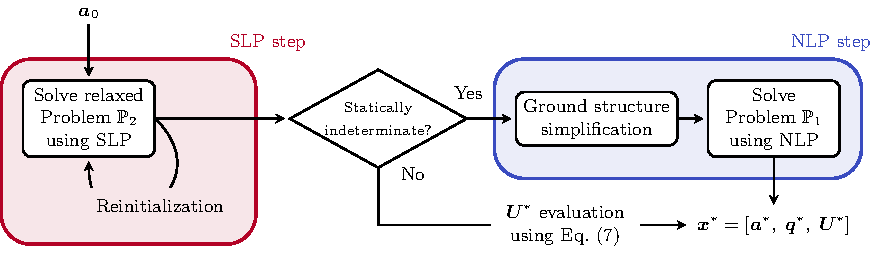
\includegraphics[width=\textwidth]{figures/04_TTO_improvements/02_solution_algo/sol_algo.pdf}
    \caption{Flowchart of the two-step optimization strategy used to solve Problem \eqrefnotext{eq:optim_complete}.}
    \label{fig:sol_alg}
\end{figure*}

\subsection{First step: SLP optimization}
The first step of the proposed optimization strategy is here described in detail. The relaxed Problem $\mathbb{P}_2$ obtained by omitting \eqrefnotext{eq:compatib} and the displacements $\vect{U}$ in Formulation \eqrefnotext{eq:optim_complete} is stated as:
\begin{equation}
    \begin{aligned}
    \min_{\vect{a}, \vect{q}^0, \dots, \vect{q}^P}  && V &= \vect{\ell}^{T}\vect{a}\\
    \textrm{s.t.}   && \matr{B}\vect{q}^p &= \vect{f}^p && \forall p \in [0,\dots,N_p]\\
    && \vect{q}^p &\geq -\frac{s\vect{a}^2}{\vect{\ell^{*2}}} && \forall p \in [0,\dots,N_p] \\
    && -\sigma_c\vect{a} &\leq \vect{q}^p \leq \sigma_t\vect{a} && \forall p \in [0,\dots,N_p] \\
    && a_{r}&\geq a_{r=1} && r \in \mathcal{C}_{l,r}(\vect{a}) \\
    && \vect{a} &\geq 0. \\
    \end{aligned}
    \tag{$\mathbb{P}_2$}
    \label{eq:optim_no_constr}
\end{equation}

Since the objective function and all of its constraints are linear, except for the buckling constraint, this problem is solved by iteratively linearizing the non-linear buckling constraints and using a \gls{slp} algorithm. Following the work of \sidecite{schwarz_efficient_2018}, the Euler's critical load is iteratively updated using a first-order Taylor expansion for every $j$ member with cross-sectional area $a_{j}^i$ at the iteration $i$ in the neighborhood of the point $\vect{P}_{i}$ (see \figref{fig:SLP}):
\begin{equation}
    \tilde{q}_{i,j}^{\text{cr}} = q_{i,j}^{\text{cr}}(a_{j}^i) + (a_{j}^{i+1} - a_{j}^i)\left.\derfrac{q_{i,j}^{\text{cr}}(a_{j}^i)}{a}\right\rvert_{a=a_{j}^i}
\end{equation}
where $a_{j}^{i+1}$ represent the design variable of the \gls{slp} at the current iteration and $q^{\text{cr}}_{i,j}(a_{j}^i) = -s ({a_{j}^i})^2/\ell^{*2}_j$ represents the Euler's critical load with cross-sectional area $a_{j}^i$ and modified buckling length $\ell^{*}_j$. 

The linearized local buckling constraints $\vect{\tilde{g}}_{\textrm{buck}}$ are then stated as:
\begin{equation}
    q_{j} \geq \tilde{q}^{\text{cr}}_{i,j},\text{ with } \tilde{q}^{\text{cr}}_{i,j}= - \frac{s a_{j}^i\left(2 a_{j}^{i+1} - a_{j}^i\right)}{\ell^{*2}_j} \quad \forall j \in [1,\ldots, N_{\text{el}}],
    \label{eq:buck_con_lin}
    \tag{$\vect{\tilde{g}}_{\textrm{buck}}$}
\end{equation}
where superscript $\sim$ indicates linearized functions and corresponding variables.

\begin{figure}
    \centering
    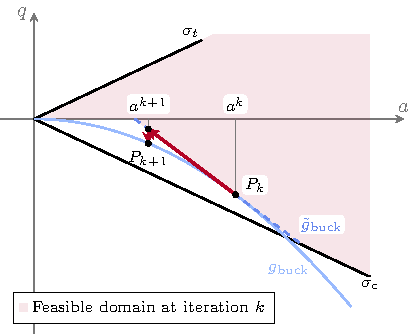
\includegraphics[width=0.5\textwidth]{figures/04_TTO_improvements/03_SLP/slp.pdf}
    \caption{\todo{magari mettila nel margin} Linearization of the local buckling constraints for a single bar.}
    \label{fig:SLP}
\end{figure}


We can now state the relaxed linearized sub-problem $\tilde{\mathbb{P}}_2$ obtained substituting \eqrefnotext{eq:buck} with \eqrefnotext{eq:buck_con_lin} in Formulation \eqrefnotext{eq:optim_no_constr}:
\begin{equation}
    \begin{aligned}
    \min_{\vect{a}, \vect{q}^0, \dots, \vect{q}^P}   && V &= \vect{\ell}^{T}\vect{a}\\
    \textrm{s.t.}   && \matr{B}\vect{q}^p &= \vect{f}^p && \forall p \in [0,\dots,N_p]\\
    && \vect{q}^p \geq - &\frac{s \vect{a}^i\left(2 \vect{a}^{i+1} - \vect{a}^i\right)}{\vect{\ell}^{*2}} && \forall p \in [0,\dots,N_p] \\
    && -\sigma_c\vect{a} &\leq \vect{q}^p \leq \sigma_t\vect{a} && \forall p \in [0,\dots,N_p] \\
    && a_{r}&\geq a_{r=1} && r \in \mathcal{C}_{l,r}(\vect{a}) \\
    && \vect{a} &\geq 0. \\
    \end{aligned}
    \tag{$\tilde{\mathbb{P}}_2$}
    \label{eq:optim_no_constr_lp}
\end{equation}

Since the objective function and all of its constraints are linear, we can approximate the solution of \eqrefnotext{eq:optim_no_constr} by iteratively solving the sub-problem \eqrefnotext{eq:optim_no_constr_lp}. At every iteration $i$, the vector of cross-sectional areas $\vect{a}^i$ is used to evaluate the linearization point $\vect{P}_{i}$ and calculate the set of linearized buckling constraints $\vect{\tilde{g}}_{\textrm{buck}}$ (see \figref{fig:SLP}). The sub-problem \eqrefnotext{eq:optim_no_constr_lp} is, then, solved using a \gls{lp} solver, and the updated vector of cross-sectional areas $\vect{a}^{i+1}$ is used to evaluate the set of linearized buckling constraints of the $i+1$ iteration. These steps are repeated until convergence \ie when $\norm{\Delta \vect{x}}_\infty\leq \text{tol}_{slp}$, where $\Delta \vect{x}$ represents the difference of the design variable vector $\vect{x}$ between two successive iterations. The vector $\vect{x}$ is scaled so that the difference $\Delta \vect{x}$ gives coherent results for the different physical quantities (cross-sectional areas and forces). \todo{Major details on scaling are given in Appendix.}

\subsection{Handling local minima: reinitialization strategy}

\subsection{Second step: NLP optimization}

\section{Numerical application}

\subsection{L-shaped beam}

To assess the effectiveness of the proposed minimum slenderness limit, we conducted a new round of optimization on the L-shaped beam described in \secref{sec:03_applications}. Formulation \ref{eq:03_optim_original} is modified adding an upper bound on the cross-sectional section based on \ref{eq:04_slend_constraints}. In the \figref{fig:04_tto_slend}, we present the optimized structures obtained using this modified formulation and the stress limits $\sigma_\text{L}$ values of 1, 0.8, 0.3, and 0.2. The first two values have already been used and the results presented in \tabref{tab:03_TTO_results}. They highligted the limits of Formulation \ref{eq:03_optim_original} when imposing a specified slenderness limit ($\lambda<15$). The last two values are introduced here to test how the \ref{eq:04_slend_constraints} constraint affect the truss topology for extreme cases. 

Major focus is put on the shorter bar of the optimized structures to observe how the solution evolved. We observe a redistribution of the same load across multiple smaller bars. More bars became active because there is an upper limit on the cross-sectional area (and thus the force) they can withstand. The four structures present $N_\text{el,sl}=34$, 38, 56 and 79 active bars, respectively.

\begin{figure*}[]
    \subcaptionbox{}{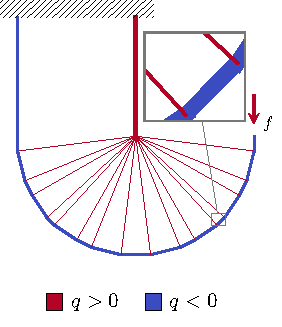
\includegraphics[width=0.23\linewidth ]{figures/04_TTO_improvements/00_slend_sol/1_opt.pdf}}
    \hfill
    \subcaptionbox{}{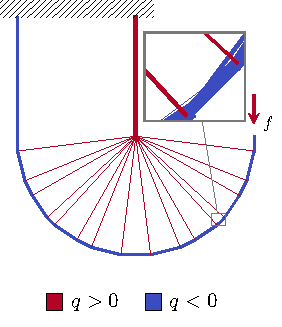
\includegraphics[width=0.23\linewidth ]{figures/04_TTO_improvements/00_slend_sol/08_opt.pdf}}
    \hfill
    \subcaptionbox{}{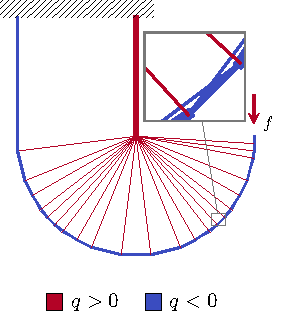
\includegraphics[width=0.23\linewidth ]{figures/04_TTO_improvements/00_slend_sol/03_opt.pdf}}
    \hfill
    \subcaptionbox{}{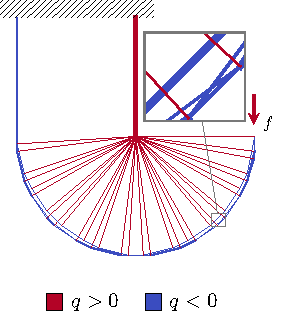
\includegraphics[width=0.23\linewidth ]{figures/04_TTO_improvements/00_slend_sol/02_opt.pdf}}
    \caption{Topology of the optimized truss structures for different material admissibles $\sigma_\text{L}=1.0,0.8,0.3\text{ and }0.2$ with a minimum slenderness limit $\lambda<15$.}
    \label{fig:04_tto_slend}
\end{figure*}

In \tabref{tab:04_TTO_l_slend} we compared the new designs limited in minimum slenderness (noted in the table with the 'sl' subscript) to the ones presented in \secref{sec:03_applications} and found that the new designs meet the bar model's slenderness requirements correctly. The number of active bars increases along with the calculation time, but the volume remains nearly the same, indicating there are many solutions with similar volumes. Adding this upper bound constraint, we have extended the domain of application of the \gls{tto}. However, we must be careful because very high volumes fraction solutions can lead to too many bar intersections, resulting in structures with no physical meaning.

\begin{table*}[]
    \centering
    \sisetup{table-auto-round}
    \begin{tabular}{S[table-format = 2.1]
                    S[table-format = 2.2]
                    S[table-format = 2.1] 
                    S[table-format = 2.2]
                    S[table-format = 2.1]                    
                    S[table-format = 1.4]
                    S[table-format = 1.2]
                    S[table-format = 1.2]}
                    \toprule
    $\bm \sigma_L$&$\bm V_\text{f}$  & {\textbf{Min} $\bm \lambda$} & $\bm V_\text{f,sl}$  & {\textbf{Min} $\bm \lambda_\text{sl}$}&$\bm V_\text{f,sl}/\bm V_\text{f}$&$\bm N_\text{el,sl}/\bm N_\text{el}$&$\bm t_\text{sl}/\bm t$\\ \midrule
    1           & 6.208431\ppercent  & 15.795                    & 6.208431\ppercent& 15.795  &1&1       &1.02            \\
    0.90        & 6.898257\ppercent  & 14.984                    & 6.898257\ppercent& 14.984  &1&1       &1.03            \\
    0.80        & 7.760539\ppercent  & \color{accent_r_1}14.127  & 7.761069\ppercent& 15.0    &1,0000682&1,1176       & 2.27    \\
    0.70        & 8.869187\ppercent  & \color{accent_r_1}13.215  & 8.870386\ppercent& 15.0    &1,0001351&1,1176       & 2.21    \\
    0.60        & 10.347385\ppercent & \color{accent_r_1}12.235  &10.349476\ppercent& 15.0    &1,0002020&1,1176      & 1.12    \\
    0.50        & 12.416862\ppercent & \color{accent_r_1}11.169  &12.420203\ppercent& 15.0    &1,0002690&1,1176      & 1.07    \\
    0.4         & {--}      & {--}                               &15.526292\ppercent& 15.0    &{--}&{--} &{--}                 \\
    0.3         & {--}      & {--}                               &20.705531\ppercent& 15.0    &{--}&{--} &{--}        \\ 
    0.2         & {--}      & {--}                               &31.061628\ppercent& 15.0    &{--}&{--} &{--}                \\ \bottomrule
    \end{tabular}
    \caption{\todo{todo}}
    \label{tab:04_TTO_l_slend}
\end{table*}

\subsection{Ten-bar truss}

\subsection{2D cantilever beam}

\subsection{Simply supported 3D beam}

\subsection{Ten-bar truss with multiple load cases}

\section{Conclusion}

\section{temporary}
\begin{figure*}[]
    \hspace*{\fill}
    \subcaptionbox{}{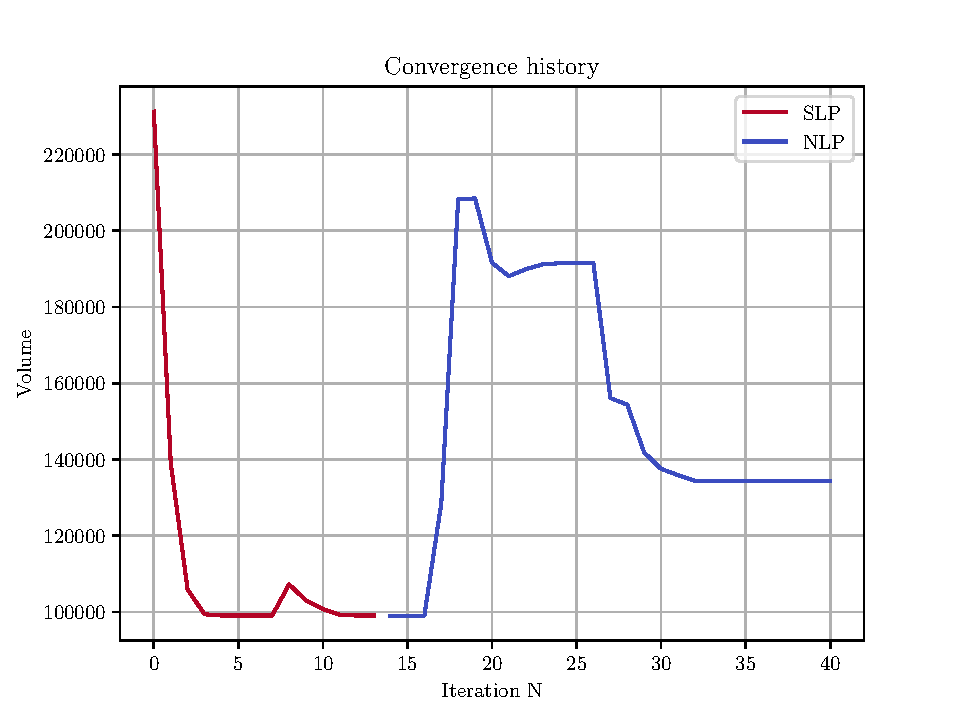
\includegraphics[width=0.45\linewidth]{figures/99_temp/01_History/01_tenbar_multipleloads/fig11_obj_hist_comb.pdf}}
    \hfill
    \subcaptionbox{}{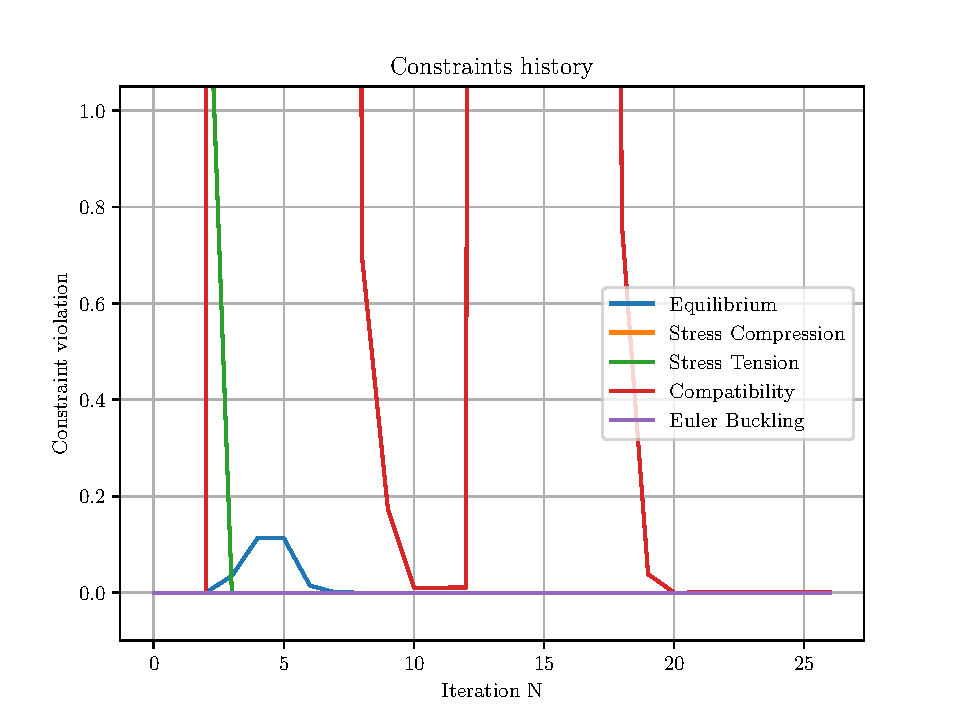
\includegraphics[width=0.45\linewidth]{figures/99_temp/01_History/01_tenbar_multipleloads/fig12_constr_hist.pdf}}
    \hspace*{\fill}
    \caption{Iteration history of the ten-bar truss with multiple load cases example solved with the 2S-1R algorithm; (a) objective function history for the SLP and NLP step (b) constraint violation for the NLP step.}
    \label{fig:}
\end{figure*}

\begin{figure*}[]
    \hspace*{\fill}
    \subcaptionbox{}{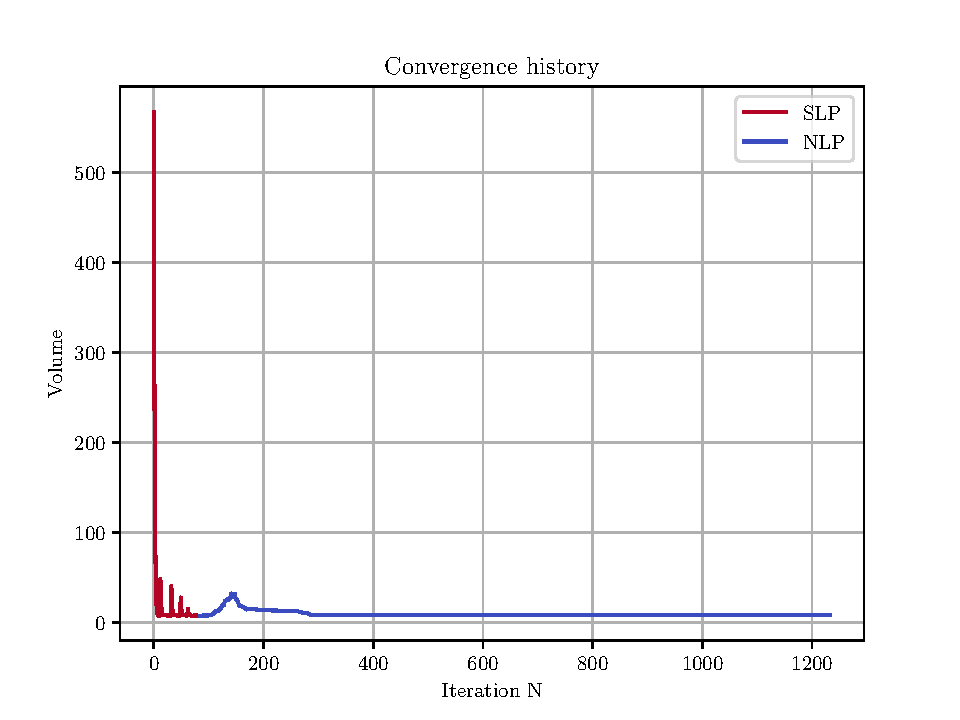
\includegraphics[width=0.45\linewidth]{figures/99_temp/01_History/02_CRM315/fig11_obj_hist_comb.pdf}}
    \hfill
    \subcaptionbox{}{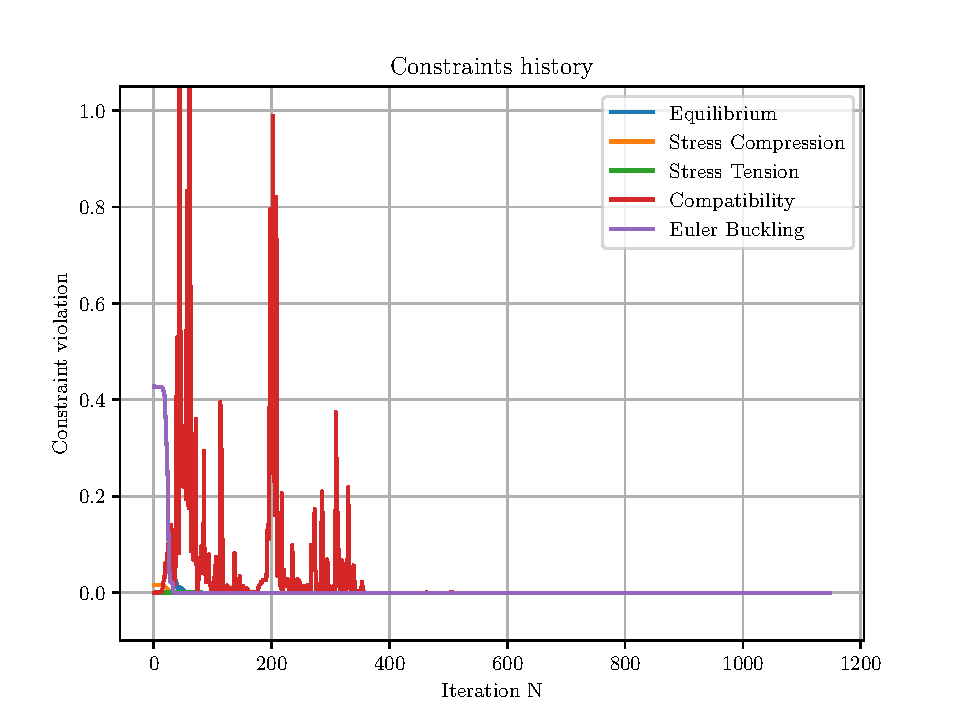
\includegraphics[width=0.45\linewidth]{figures/99_temp/01_History/02_CRM315/fig12_constr_hist.pdf}}
    \hspace*{\fill}
    \caption{Iteration history of the CRM-315 example solved with the 2S-5R algorithm; (a) objective function history for the SLP and NLP step (b) constraint violation for the NLP step.}
    \label{fig:}
\end{figure*}

\begin{figure*}[]
    \hspace*{\fill}
    \subcaptionbox{}{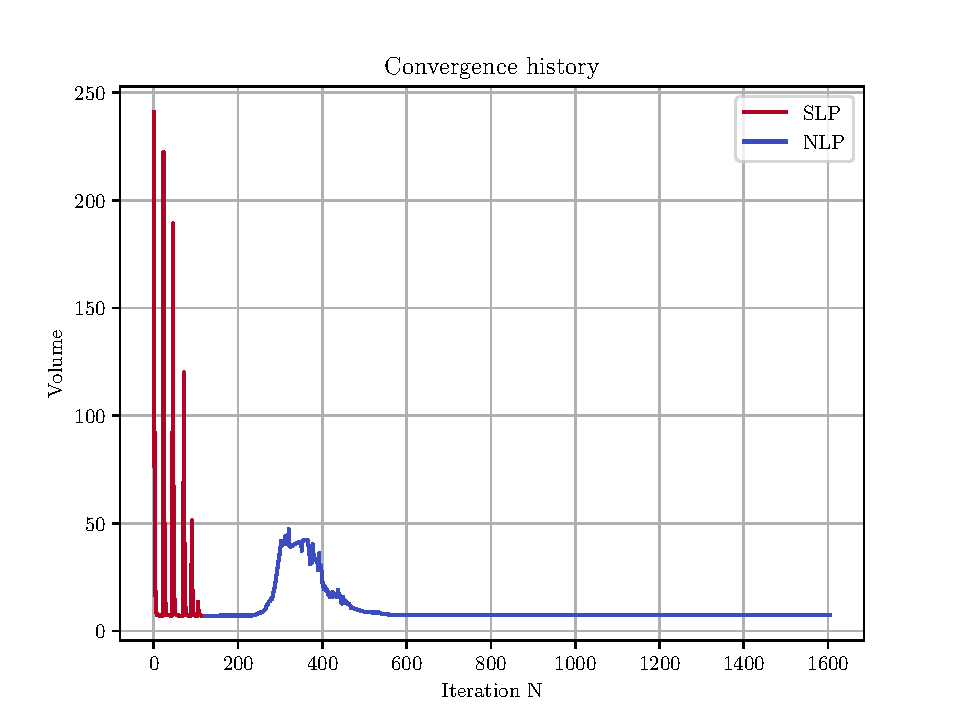
\includegraphics[width=0.45\linewidth]{figures/99_temp/01_History/03_CRM2370/fig11_obj_hist_comb.pdf}}
    \hfill
    \subcaptionbox{}{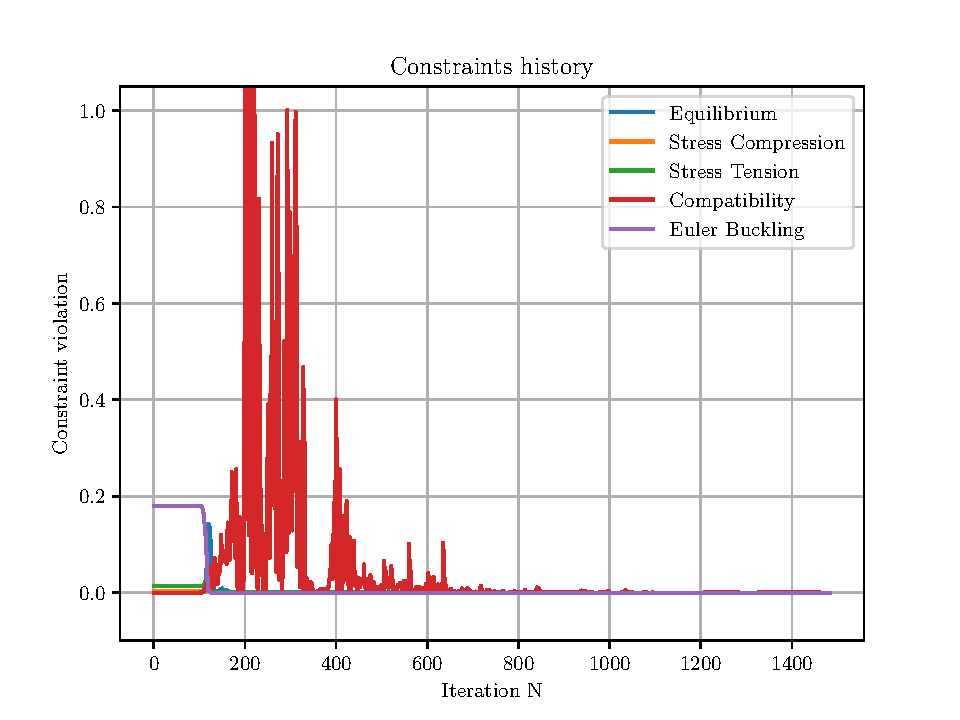
\includegraphics[width=0.45\linewidth]{figures/99_temp/01_History/03_CRM2370/fig12_constr_hist.pdf}}
    \hspace*{\fill}
    \caption{Iteration history of the CRM-2370 example solved with the 2S-5R algorithm; (a) objective function history for the SLP and NLP step (b) constraint violation for the NLP step.}
    \label{fig:}
\end{figure*}
 